\begin{frame}
\frametitle{Data and representation}

   \begin{center}
   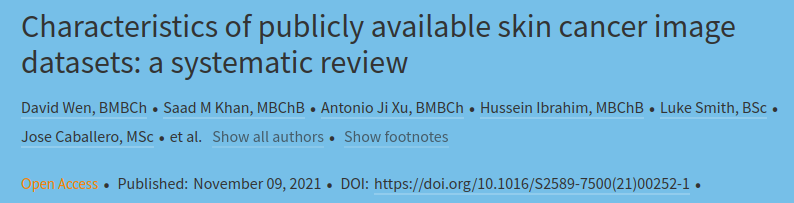
\includegraphics[width=1.0\textwidth]{./misc_images/skin-1}
   \end{center}
\vspace{1mm}
\textit{`This is the first systematic review to characterise publicly available skin image datasets, highlighting limited applicability to real-life clinical settings and restricted population representation, precluding generalisability'}
\vspace{2mm}

The data used to train a model is usually more important than the details of the machine learning method used, so before using AI in healthcare ask whether the training data is representative of the real-world clinical setting.
\end{frame}